\documentclass[a4paper,11pt,onecolumn,final,openright]{report}

\usepackage[utf8]{inputenc}
\usepackage{subfigure}
\usepackage[english]{babel}
%\usepackage{natbib}
\usepackage[T1]{fontenc}
\usepackage{graphicx}
\usepackage{float}
\usepackage{booktabs}
\usepackage{url}
\usepackage{xcolor}  
\usepackage{verbatim}
\usepackage{hyperref}
\usepackage{parcolumns}
\usepackage{fancyvrb}
\usepackage{verbatimbox}
\usepackage{threeparttable}
\usepackage{acronym}
\usepackage{listings}
\usepackage{textcomp}
\usepackage{pdflscape}
\usepackage[title]{appendix}

%%%%%%%%%%%%%%% LUA SCRIPTING FOR LSTLISTING CODES! %%%%%%%%%%%%%%%%%
\lstdefinelanguage{Lua} 
{
        basicstyle       = \footnotesize,
        backgroundcolor=\color{white!95!black},
        morekeywords={and,break,do,else,elseif,end,false,for,function,if,in,local,nil,not,or,repeat,return,then,true,until,while,_G,_ENV,io,read,write}, 
        sensitive=false, 
        morecomment=[l]{--}, 
        morecomment=[s]{--[[}{]]}, 
        morestring=[b]",
        upquote=true,
        breaklines=true,
        frame=tb,
        captionpos=b,
        showstringspaces=false,
        morestring=[b]' 
}

%%%%%%%%%%%%%%% DIFF FILES FOR LSTLISTING CODES! %%%%%%%%%%%%%%%%%
\lstdefinelanguage{diff}{
  backgroundcolor=\color{white!95!black},
  basicstyle=\footnotesize,
  showstringspaces=false,
  upquote=true,
  breaklines=true,
  frame=tb,
  captionpos=b,
  morecomment=[f][\color{blue}]{@@},     % group identifier
  morecomment=[f][\color{green!50!black}][0]>,         % deleted lines 
  morecomment=[f][\color{red!60!black}][0]<,       % added lines
  morecomment=[f][\color{black}]{---}, % Diff header lines (must appear after +,-)
  morecomment=[f][\color{magenta}]{+++},
}

%%%%%%%%%%%%%%% BASH FILES FOR LSTLISTING CODES! %%%%%%%%%%%%%%%%%
\lstdefinelanguage{bash}{
  backgroundcolor=\color{white!95!black},
  basicstyle={\footnotesize\ttfamily},
  breakatwhitespace=true,
  breaklines=true,
  captionpos=b,
  frame=tb,
  resetmargins=true,
  sensitive=true,
  stepnumber=1,
  tabsize=4,
  upquote=true
}

%%%%%%%%%%%%%%%%%%%%%%%%%%%%%%%%%%%%%%%%%%%%%%%%%%%%%%%%%%%%%%%%%%%%%%

%Reset footnote number each chapter
\makeatletter
\@addtoreset{footnote}{chapter}
\makeatother

\begin{document} 
\begin{titlepage}
    \centering
    \vspace*{\baselineskip}
    \rule{\textwidth}{1.6pt}\vspace*{-\baselineskip}\vspace*{2pt}
    \rule{\textwidth}{0.4pt}\\[\baselineskip]
    {\LARGE LEDE Firmware optimization for wired deployments using BGP and BMX6 for routing by enhancing and extending Bird Daemon's configuration and UI integration}
    \rule{\textwidth}{0.4pt}\vspace*{-\baselineskip}\vspace{3.2pt}
    \rule{\textwidth}{1.6pt}\\[\baselineskip]
    \scshape
    Theale, June 2017\par
    \vspace*{2\baselineskip}
    Major: Computer Science\par
    Minor: Open Source Software\par
    \vspace*{2\baselineskip}
    Author: \\
    {\Large Eloi Carb\'{o} Sol\'{e}\par}
    \vspace*{1\baselineskip}
    External consultant: \\
    {\large V\'{i}ctor Oncins Biosca\par}
    Routek SL\par
    \vspace*{1\baselineskip}
    Director: \\ 
    {\large Joan Manuel Marqu\`{e}s Puig\par}
    Computer Science, Multimedia and Telecomunications Department (DPCS-ICSO)
    \vfill
    \begin{figure}[ht!]
        \centering
        
\includegraphics[width=0.6\textwidth]{images/logo}
	\end{figure}
    {\large Universitat Oberta de Catalunya}\par
    {\scshape 2017}
\end{titlepage}

\newpage
\chapter*{Project Key Data}

\begin{table}[htbp]
\centering
\begin{tabular}{|>{\columncolor[gray]{0.8}}p{3.7cm}|p{9cm}|}
\hline
Títol del treball: & Optimització del Firmware LEDE per desplegaments basats en xarxes cablejades utilitzant BIRD Daemode la integració gràfica de la configuració BIRD-BMX i anàlisis respecte desplegaments en Quagga \\ \hline
Project's Title: & LEDE Firmware optimization for wired deployments using BGP (Bird Daemon) and BMX for routing by enhancing and extending Bird Daemon's configuration and UI integration \\ \hline
Nom de l'autor: & Eloi Carb\'{o} Sol\'{e} \\ \hline
Nom del consultor: & Víctor Oncins Biosca \\ \hline
Data de lliurament: & 06/2017\\ \hline
\`{A}rea del Treball Final: & Sistemes Distribu\"{i}ts \\ \hline
Titulació: & M\`{a}ster Universitari en Programari Lliure \\ \hline
\end{tabular}
\end{table}

\newpage
\section*{Resum del Projecte}
\thispagestyle{empty}
En aquest treball s'ha 




\noindent\rule{\textwidth}{0.4pt}

\section*{Abstract}
\thispagestyle{empty}

lorem ipsum

\noindent\rule{\textwidth}{0.4pt}

\newpage
\chapter*{Acknowledgements}
\thispagestyle{empty}

stuff

\cleardoublepage

\pagestyle{plain}
\pagenumbering{roman}


\def\contentsname{Index}
\tableofcontents
\newpage

\listoffigures
\newpage
\lstlistoflistings
\newpage


\chapter{Introduction}
\label{ch:introduction}
\pagenumbering{arabic}
\pagestyle{headings}

\section{Structure of the document}
%%%TBD

\section{Motivation and description of the problem}
\label{sec:bdotp}
This project aims to simplify and enhance management and monitoring capabilities of network administrators' using Bird Daemon software on top of an OpenWRT/LEDE-based Firmware. This project is a second iteration in the development of an existing configuration integration package already being used by OpenWRT/LEDE's community.

\subsection{Motivation}
Back in 2014, while working on my BSc. dissertation in the \textit{Universitat Politècnica de Catalunya}, the department and, specifically, the investigation team I was working with, gave me the opportunity to participate in a GSoC\footnote{Google Summer of Code (\href{https://www.google-melange.com/archive/gsoc/2014/orgs/freifunk/projects/eloicaso.html}{2014})} project under the umbrella of Freifunk, to design, develop and present  a package that would help simplifying the configuration of Bird Daemon as a software able to share routes between BMX6 meshs and BGP infrastructure networks deployed in \textit{frontier} nodes deployed in the Catalan community network Guifi.net.

That project was successful and the result was an integration package using OpenWRT's well-known UCI/LUCI configuration mechanism to set up Bird through a user-friendly Web UI even without deep knowledge of Bird's syntax. GSoC's time frame though was not enough to polish the package and add some secondary protocols and the package stopped getting maintenance from myself later that year. However, it has been an OSS project that has been on my \textit{backlog} of things I want to keep improving and also been queried some times by Víctor Oncins as it is really helpful for network administrators but it is not mature enough for complex production environments available in Guifi.net.

Therefore, I have been really lucky to have the opportunity to retake this package as my MSc. project while doing my MSc. and work together Víctor as this has meant that I have had direct feedback from administrators using the tool in production environments and to improve its most critical features. Moreover, Víctor has also published a report on GitHub \cite{bgpbmx6} describing the main challenges found using the old version of the Package and a deep description of the environment.

\subsection{Bird Daemon}
Bird Daemon, from now onwards Bird, is an open source Internet Routing service (daemon) that allows network administrators to simplify route sharing configuration, management and monitoring by using Routing tables and a powerful filtering language\footnote{Bird Daemon: \href{http://bird.network.cz/}{Link}}.

\subsection{OpenWRT/LEDE's configuration integration package}
Bird-OpenWRT Package, from now onwards \textit{the Package}, is an open source OpenWRT/LEDE-specific solution (\textit{.ipk}) integrated by four separated packages (two for Bird IPv4 (\textit{bird4-uci}) and IPv6 (\textit{bird6-uci}) UCI integration and the other two for Web UI management (\textit{luci-app-bird4} and \textit{luci-app-bird6}) providing Bird Daemon a user-friendly configuration scheme (UCI) and a graphical interface in OpenWRT/LEDE-based routers.

\subsection{Bird Daemon administration issues}
\label{subsec:bdai}
As part of the GSoC project, the solution provided was not mature enough to fulfil all the requirements:
\begin{itemize}
    \item Tight time-frame forcing to prioritise the key capabilities to implement.
    \item Some key protocols were not enabled in the final solution because they were not relevant for GSoC's scope (i.e. Pipe or Direct).
    \item Some secondary protocols were not enabled in the final solution because they were not relevant for GSoC's scope (i.e. OSPF or )
    \item Some basic processes require manual (terminal) changes
    \item No possible way to edit Filters or Functions files through Web UI.
    \item No Bird Daemon Status feedback (i.e. no way to know if bird is running or failed to start through Web UI).
    \item No possible way to see Bird Daemon's Log information through Web UI.
    \item Bird's API changed (from Bird 1.4.3 to 1.6.3) making bird crash using base Package configuration
    \item No possible way of monitoring Bird's current status (i.e. full information for BGP connections)
\end{itemize}
\section{Scope of the project}
\label{sec:sotp}
This project's scope is to adopt as many of the mentioned enhancements that are clearly aligned with eradicating required manual changes in command line, improve the UX\footnote{UX: User eXperience} and to align the packet with current Bird Daemon API in the given time frame of 3 months. As a result of a \textit{backlog} prioritization, the following items were agreed (in priority order):

\begin{itemize}
    \item Update the package to the latest Bird API.
    \item Update old version's disruptive issues (i.e. disabled Protocols).
    \item Status, Log, Filters and Functions Graphical integration.
    \item Theoretical viability investigation of uBus integration.
\end{itemize}


\subsection{Deviations from the original plan and future  work}
While agreeing the original scope of the project, few extra ideas and tasks were planned but, as a matter of priorities and time constraints, some were dismissed or set as future work.

\begin{itemize}
    \item Add secondary protocols: adopt more key features from Bird and increasing the range of administrators being able to take advantage of this Package.
    \item Integrate next generation of Web UI using LUCI2: HTML/JavaScript-based UI instead of LUA-based.
    \item Implementation of uBus integration according to the results of the investigation done in this project.
    \item Comparative set of tests between Quagga and Bird Daemon solutions.
\end{itemize}

Most of these extra tasks are already documented as part of the Package Documentation Reporitory\footnote{GitHub TODO List: \href{https://github.com/eloicaso/bgp-bmx6-bird-docn/blob/master/EN/TODO.md}{Link}.} and open for discussion and Pull Requests\footnote{Pull Request: Changes pushed to a repository by an external party (i.e. a fork repository pushing changes to its parent.} to add extra requirements.

\subsubsection{Bird Daemon VS. Quagga deployments}
There is a special reasoning behind not doing a comparative analysis of these two solutions. Of course, the timing constrains have strongly influenced the decision of dropping it from this project's scope, but there is also the big amount of evidence already collected for my GSoC project as well as some new evidence found either in some reputable sources as well as from Bird's own OSS Community proving that Bird Daemon has been far more stable, less resource eater and flexible (thanks to its Filter\&Function scripting language) than other well-known enterprise level solutions. This evidence is available in the Appendix \ref{app:ch:blinks}.


\subsection{Methodology and communication}
This project starts with the premise that there is no need for a wide initial investigation phase as the Package used was designed and developed by myself. Nevertheless, there are three foreseen introductory tasks:
\begin{itemize}
    \item Refresh the Package to the latest Bird Daemon version API. 
    \item Investigate, understand and document the production environment.
    \item Update Documentation and prepare the repositories required (documentation, package and dissertation).
\end{itemize}

After this initial phase, the implementation tasks will be executed in a Kanban-like approach:
\begin{itemize}
    \item Features will be executed following Backlog's priority order and one at a time.
    \item Each \textit{feature}/\textit{requirement} must be self-contained and the Package should be releasable at any time.
    \item There is no Board or framework to introduce the data (i.e. time spent or state of the tasks) as such as the overhead of doing it is not proportional to the number of tasks or value of the data that could be collected. However, during the first \textit{Cycle} of the project (first two weeks), in order to illustrate how could this project look like using Kanban, I did use an online OSS tool called \textit{Taiga.io}\footnote{\href{https://taiga.io/}{Taiga.io}: Online project management tool working either with Kanban or SCRUM Agile methodologies. This tool is widely used in OSS projects due to its power, simplicity and plugins (open API) and has also enterprise options.}. See Appendix \ref{app:sec:kanban} in order to see some captures of the initial tasks created using the tool.
    \item There will be weekly/bi-weekly meetings with the Stakeholder in order to discuss progress, any blocker or issue and rearrange priorities if required.
    \item There will be a \textit{demo} to the Stakeholder to show progress in a weekly/bi-weekly basis.
\end{itemize}

The communication, as already mentioned, will be done through regular meetings with the External Consultant (Stakeholder) using the Jitsi\footnote{\href{https://jitsi.org/}{Jitsi}: Open Source multiplatform VoIP conference service.} conference service, which allows screen sharing and text communication while in conference, simplifying demoing and code reviews. Regular communication will be also done through Hangouts instant messaging service and by email to share progress, risks or blockers.

\subsubsection{Gantt Diagram}
Tasks' delivery forecast can be seen in Figures  \ref{fig:general_gantt} and \ref{fig:detail_gantt}:

\begin{landscape}

\begin{figure}[h!]
\centering
    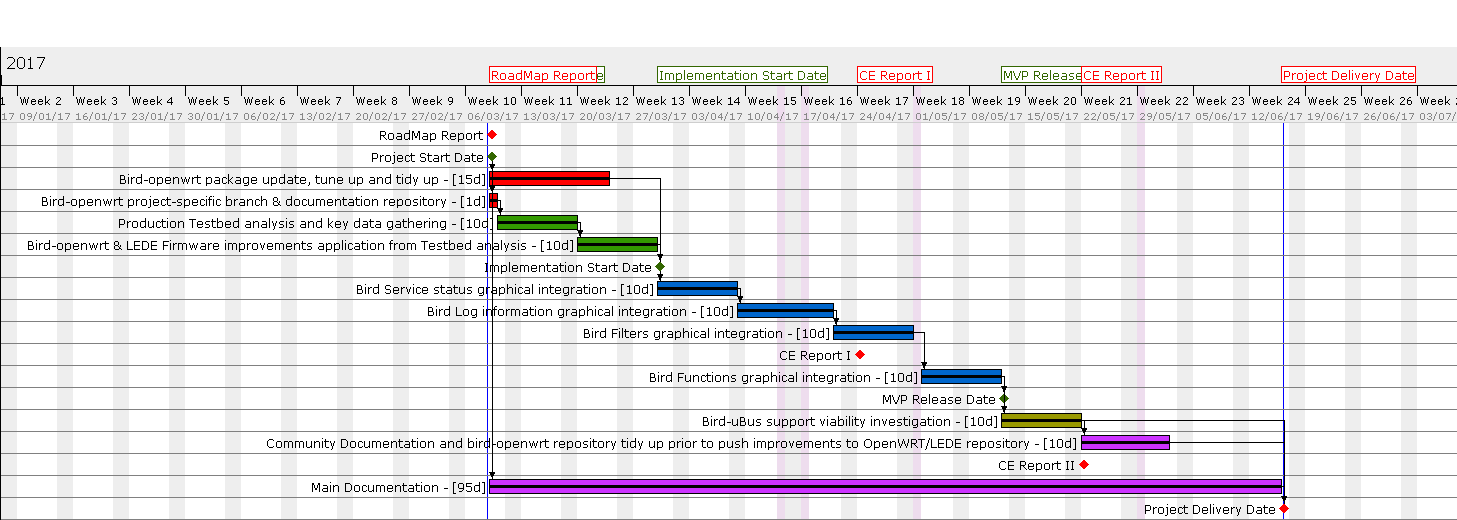
\includegraphics[width=\hsize]{images/gantt}
    \caption{Tasks schedule}
    \label{fig:general_gantt}
\end{figure}

Key milestones:
\begin{itemize}
    \item \textbf{Project's start date \& RoadMap Report} (09/03/17): initial Package refresh and production environment investigation. Formal report of which are project's goals and when are they expected to be delivered.
    \item \textbf{Project's implementation start date} (30/03/17): beginning of features' implementation.
    \item \textbf{Continuous Evaluation Report I} (22/04/17): formal report to present Project's progress, pending work, any issue or blocker and updated  timeline.
    \item \textbf{MVP Release} (12/05/2017): forecast delivery date of the final version of the Package. No extra changes planned unless the investigation task requires them.
    \item \textbf{CE Report II} (22/05/17): optional progress report prior to Project's delivery.
    \item \textbf{Project Delivery Date} (12/06/17): final date to deliver the dissertation, slides+recording and any extra archive required.
\end{itemize} 

\begin{figure}[h!]
    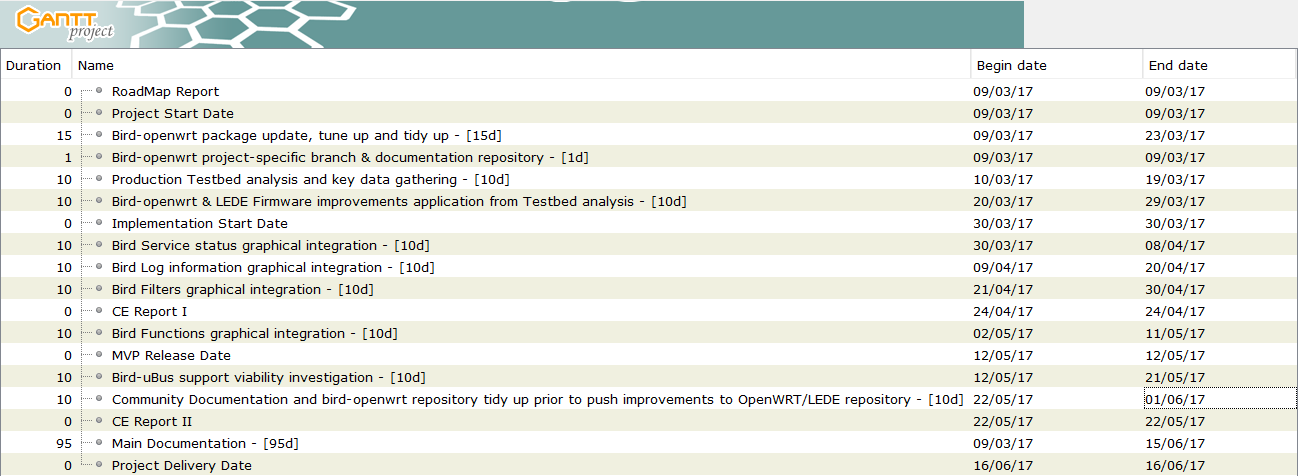
\includegraphics[width=\hsize]{images/gantt_data}
    \caption{Schedule details}
    \label{fig:detail_gantt}
\end{figure}
\end{landscape}


\section{Background information}
\label{sec:backc}
\subsection{Guifi.net}
\label{subsec:gn}
Guifi.net is a community network working for and by its own users (self-organised) giving an affordable alternative for anyone willing to connect to the Internet. This network's principles are freedom, open design, administration and management and neutrality. This network was born in Catalonia as a wireless network but it has spread all over the world and with about 33.124\footnote{Guifi.net live statistics: \href{https://guifi.net/guifi/menu/stats/nodes}{Link}} active nodes (as 26/05/17) using roof antennas and optical fiber deployments.

This network is connected to the Catalan Internet Exchange Point (CATNIX\footnote{CATNIX: \href{http://www.catnix.net/en/}{Link}}), has its own Government Foundation\footnote{Fundació Guifi.net: \href{https://fundacio.guifi.net/Foundation}{Link}} to promote and protect network's principles defined in an operational and behavioural common regulation (Comuns - XOLN\footnote{\href{https://guifi.net/en/FONNC}{XOLN/FONN}: Compact for a Free, Open \& Neutral Network}) and it is open for any company that adheres to the XOLN/FONNC principles, to professionally operate and advertise itself as a Guifi.net Internet or services provider. 

Finally, although Guifi.net main routing protocol is BGP for infrastructure and OSPF for internal routing, there are several isles\footnote{Guifi.net Mesh Networks: \href{http://ca.wiki.guifi.net/wiki/Annex:subxarxes_mesh}{Link}}\footnote{\href{http://qmp.party/Documentation}{qMp}: Most commonly used firmware in Guifi.net for mesh networks. This OpenWRT fork aims to simplify and automate mesh deployments.} operating as Mesh Networks using BMX6 dynamic routing protocol.

\subsection{OpenWRT/LEDE Project}
\label{subsec:owrtlp}
OpenWRT, and its Fork LEDE-Project\footnote{LEDE-Project: Linux Embedded Development Environment.}, are Open Source Linux-based firmwares primarily focused on commodity routers, but aiming to work in any Linux-based system. This firmware supports a wide variety of manufacturer's hardware and also a wide range of software, services and routing protocols to enhance, secure and efficiently operate as a standalone router and service provider.

\subsection{Infrastructure vs Mesh Network Routing Protocols}
\label{subsec:dsrp}
Routing protocols' job is to receive a route and, according to its attributes and the information stored in the system, to redirect this route to the next step towards its destination or to drop it. However, 

\begin{itemize}
    \item \textbf{Infrastructure}: commonly used in structural networks. Stable, robust and scalable. Their main handicap is to suffer of big overheads on topology changes (i.e. low/non fault tolerance) and have big convergence times in large-scale networks.
    \item \textbf{Mesh Networks}: oppositely to classic dynamic networks, mesh networks' strength is to be able to converge almost instantly after any topology event. These networks work in a cooperative manner in order to achieve a fully connected network (point-to-multipoint) where all the nodes share network's knowledge in order to optimise routes and nodes floods the network in order to keep the network topology knowledge up to date.
\end{itemize}

\subsubsection{BGP}
\label{subsubsec:bgp}
BGP is a dynamic infrastructure IP routing protocol designed for large-scale internet topologies (EGP\footnote{EGP: Exterior Gateway Protocol. This includes all the protocols that routes between Autonomous systems.}). Its routing algorithm relies on the best path according to route's attributes.

\subsubsection{BMX6}
\label{subsec:bmx6}
Batman-eXperimental6 \cite{bmx6} is a fork of the Mesh protocol BATMAN\footnote{\href{https://www.open-mesh.org/projects/open-mesh/wiki}{B.A.T.M.A.N}: Better Approach To Mobile Adhoc Networking.}. This is a mesh networking routing protocol is compatible with most of linux-like systems but only operates with IPv6 networks. This routing protocol uses a table-driven\footnote{Table-driven: Compose a routing table with all the source-destination entries.} distance-vector approach\footnote{Distance-vector: Best path (cost of going) from source to destination.}.


\section{State of the art}
\label{sec:soa}

\chapter{Network Architecture}
\label{ch:architecture}
\pagestyle{headings}

As shown in the figure \ref{fig:tarnet}, our targeted network is a mixed section requiring the use of Exterior Gateway Protocols (IGP) and Internal Gateway Protocols (EGP) in order be able to share routes routes between the two BGP ends (named \textit{E} and \textit{F}) going through a BMX6 Mesh Network (from report \cite{bgpbmx6} - in Catalan). 

As shown in the figure:
\begin{itemize}
    \item \textbf{Infrastructure Super Node 1} (ISN1): BGP Supernode connected to the BGP network (Guifi.net, section 1) via wireless and to the MXN1 Router through Ethernet.     
    \item \textbf{Mesh eXchange Node 1} (MXN1): LEDE/OpenWRT router connected via Ethernet to the ISN1 and to the antenna (or an Ethernet port) providing access to the Mesh Network. This frontier node provides BGP to BMX6 route-sharing capabilities using Bird Daemon.
    \item \textbf{Mesh Network}: A number of Nodes connected using BMX6 forming an isle between BGP nodes.
    \item \textbf{Mesh eXchange Node 2} (MXN2): LEDE/OpenWRT router connected via Ethernet to the ISN2 and to the antenna (or an Ethernet port) providing access to the Mesh Network. This frontier node provides BGP to BMX6 route-sharing capabilities using Bird Daemon.
    \item \textbf{Infrastructure Super Node 2} (ISN1): BGP Supernode connected to the BGP network (Guifi.net, section 2) via wireless and to the MXN2 Router through Ethernet.
\end{itemize}

\newpage

\section{Routing requirements}
Routing requirements to successfully ensure that all routes are shared between both BGP ends are:

\begin{itemize}
    \item Routes must be shared/announced between ISN1 (\textbf{E}) and ISN2 (\textbf{F}).
    \item Mesh Network's Routes (BMX6 - \textbf{C}\&\textbf{D}) must be shared/announced to ISN1 and ISN2 (\textbf{A}\&\textbf{B}). Therefore, shared/announced to Guifi.net network.
    \item ISN1 and ISN2 Routes (BGP - \textbf{A}\&\textbf{B}) must be shared/announced to the Mesh Network (\textbf{C}\&\textbf{D}).
    \item MXN1/2 must configure Bird to use a custom Routing Table that will be shared with BMX6.
    \item MXN1/2 must configure BMX6 to use the \textit{Table} plugin in order to redirect its routes from Kernel's Table to a custom one.
    \item MXN1/2 must configure Bird to set them both as BGP Peers to stablish an iBGP session between them (AS2).
    \item MXN1 must configure Bird to set ISN1 as BGP Peer AS1
    \item MXN2 must configure Bird to set ISN1 as BGP Peer AS3
\end{itemize}

\subsection{Caveats}
There is an important caveat with this network distribution:

Current version of BMX6 is not able to handle the number of routes that this Guifi.net BGP section is sharing (2.500+). Therefore, BMX6 starts aggregating routes, which eventually shut-downs the service and leaves the node overloaded as it is not able to achieve it.

In order to avoid this disruptive issue, Bird Daemon filter scripting capabilities available in MXN1 and MXN2 allow to reduce the geographical scope of the routes imported and exported to/from the Barcelon\`{e}s\footnote{\href{https://guifi.net/barcelones}{Barcelon\`{e}s}: Network Zone including Badalona, Barcelona, Hospitalet del Llobregat, Sant Adri\`{a} del Besos and Santa Coloma de Gramanet} Zone.

\begin{landscape}

\begin{figure}[ht!]
        \centering
        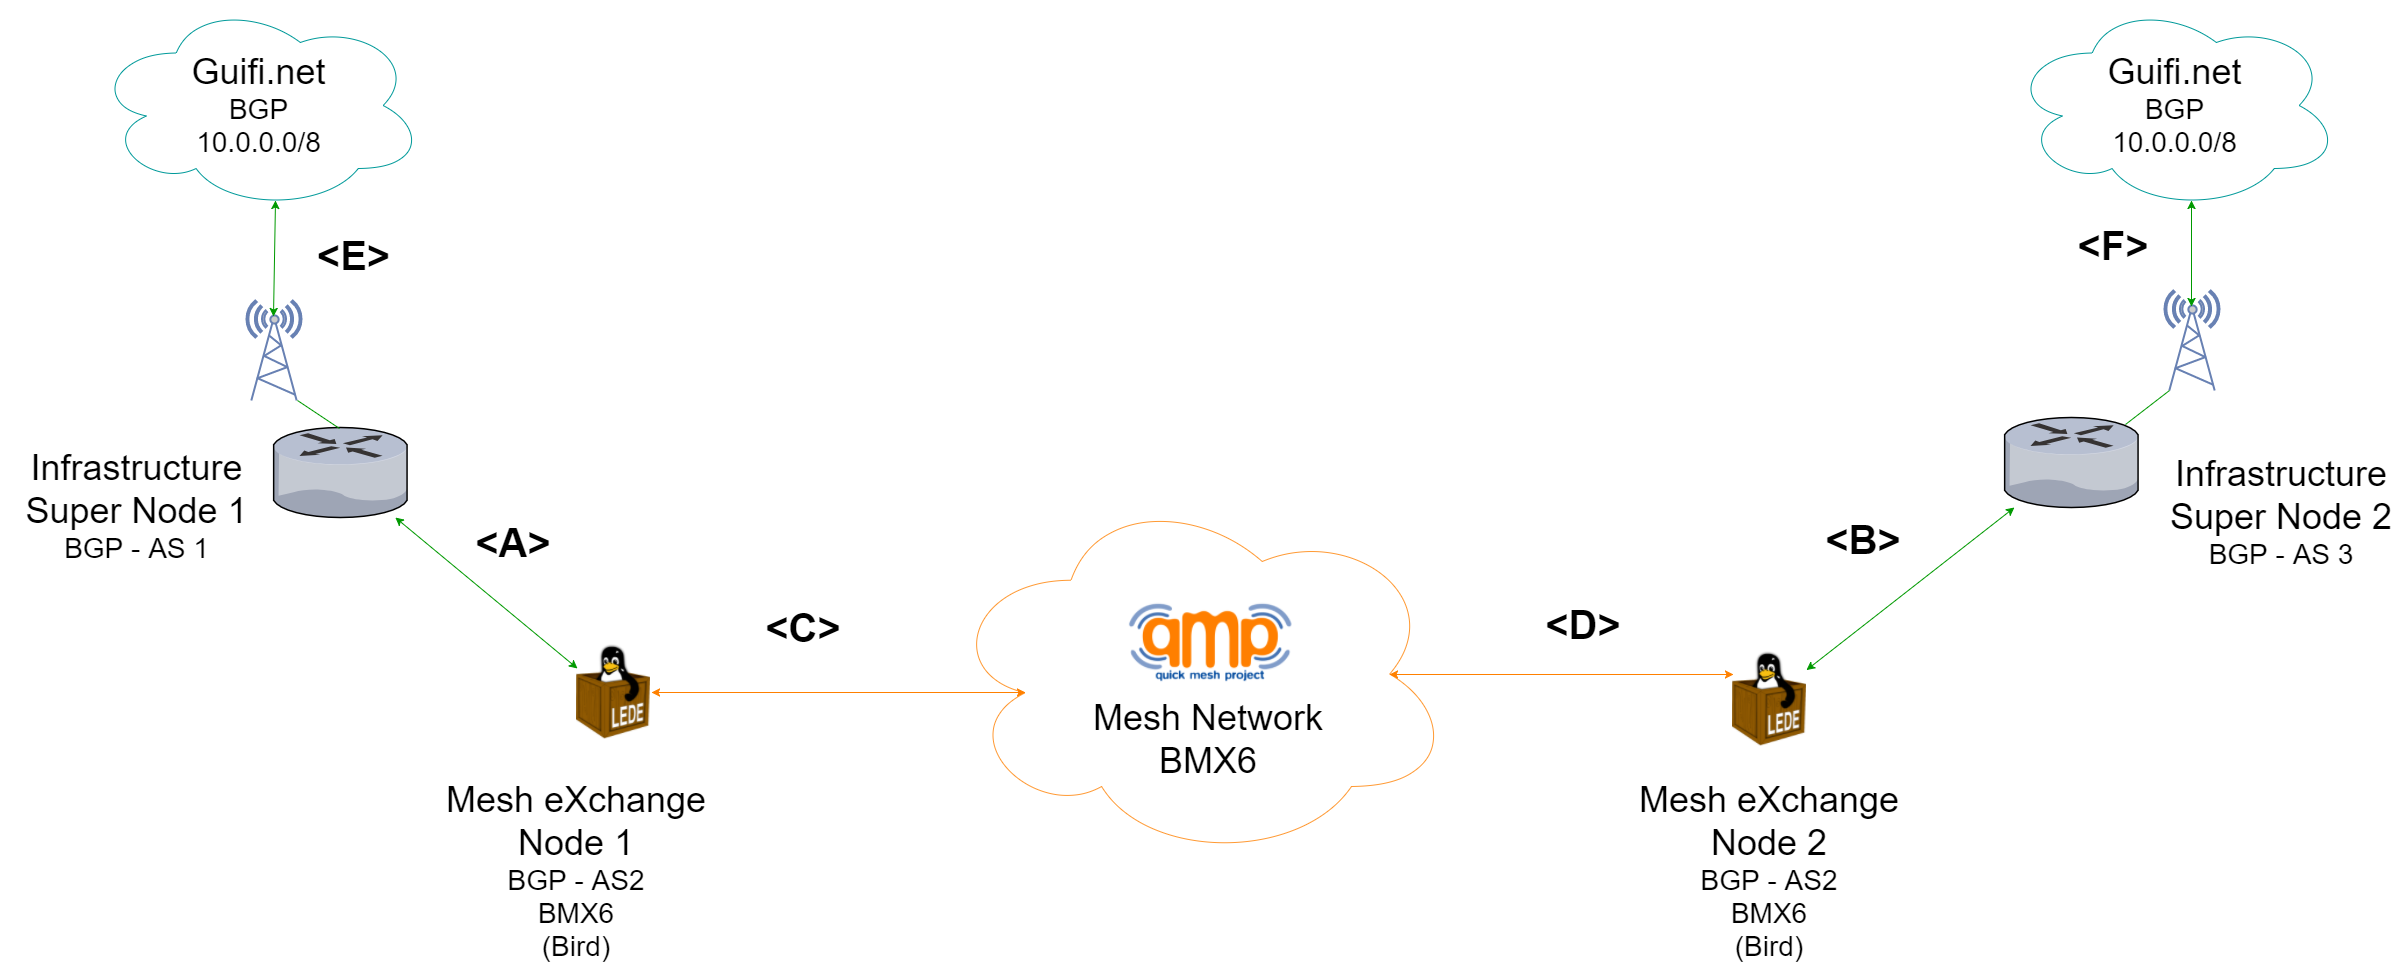
\includegraphics[width=\hsize]{images/targetnet}
        \caption{Production Network targeted in this project}
        \label{fig:tarnet}
	\end{figure}
\end{landscape}
\newpage

\section{Real environment testing}
Although it has not been possible to test Package's improvements due to the impact that a change like this could incur in a live network involving several critical \textit{Super Nodes} and all the routes in the Mesh Network, it is foreseen to be updated soon in a planned and backed up manner.

\subsection{Development environment testing}
The \textit{Universitat Oberta de Catalunya} and V\'{i}ctor have provided me a number of Virtual Machines plus a number of network resources in order to simulate our target network but without the risk of damaging the production network or flooding unwanted routes to Guifi.net.

\begin{itemize}
    \item VPN access to the Guifi Network using UOC's resources.
    \item 4 Virtual Machines using LEDE17.01 Firmware.
    \item Virtual Bridge to connect the VMs simulating a Mesh Network.
    \item Network way through two different network sections.
    \begin{itemize}
        \item Connection using UOC's Super Node
        \item Virtual Machine 4 connects through UPF\footnote{Universitat Pompeu Fabra}'s internal network to find path out to a near Guifi network.
    \end{itemize}
\end{itemize}

\begin{landscape}

\begin{figure}[ht!]
        \centering
        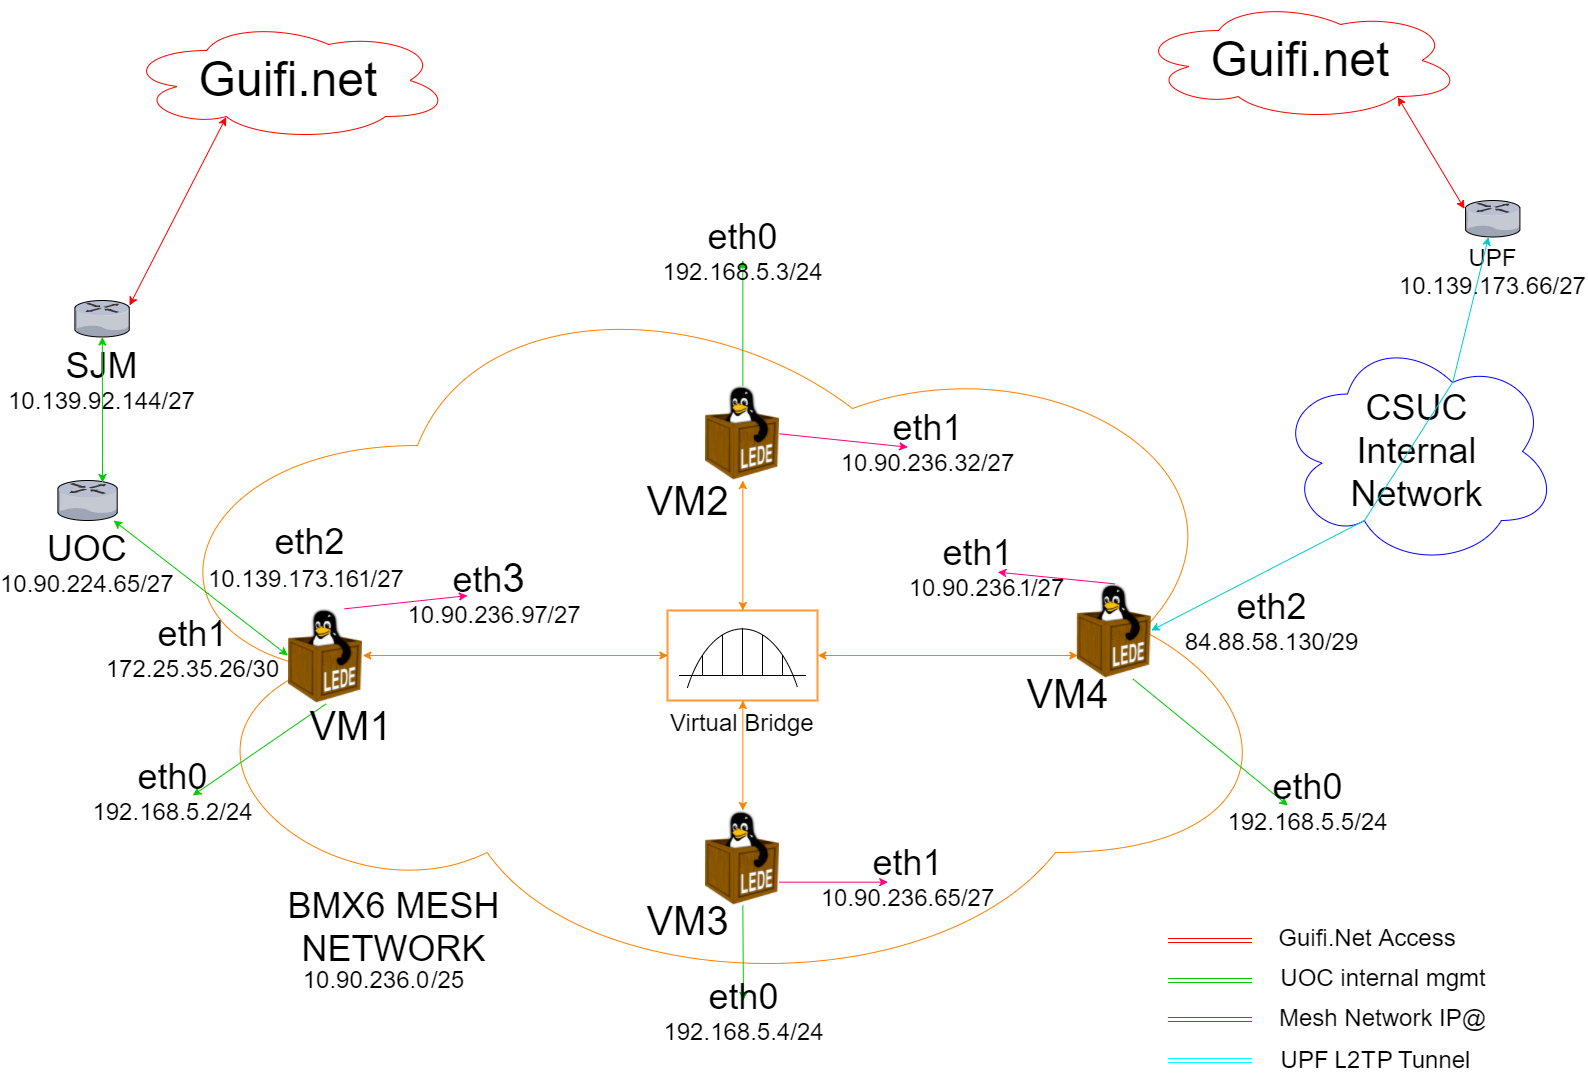
\includegraphics[width=\hsize]{images/devnetfull}
        \caption{Development Network simulating production's environment}
        \label{fig:devnet}
	\end{figure}
\end{landscape}
\newpage


\chapter{Package improvements implementation}
\label{ch:implementation}
\pagestyle{headings}

\section{Administration requirements}
One of the administrator's main tasks while managing networks is, if necessary, to facilitate the coexistence of different Routing protocols in the same network section. Hence the requirement of rich tools as Quagga or Bird to act as facilitators of this route transference between them.

Administrators require:
\begin{itemize}
    \item A full-featured tool with an easy and intuitive UI to manage and monitor protocol health and data efficiently and avoiding any handmade/custom edit, reducing configuration's complexity.
    \item Use LEDE/OpenWRT-based firmwares widely used in the target network.
    \item A Routing protocols management tool that, at least, supports BGP Static Routing Protocol and it is able to share routes with BMX6 Dynamic Routing Protocol in a manageable way.
    \item Use Bird Daemon instead of Quagga to make us of its proven efficiency, low resource consumption and powerful filter capabilities, which is critical to some of the widely used commodity hardware in Guifi.net.
    \item Use and improve Bird Daemon's configuration integration package (bird-uci and luci-app-bird) available in the official Routing Repository of LEDE/OpenWRT.
    \item Avoid project-specific customisations in the integration package that would not benefit all the community. If required, add those custom enhancements in a development branch.
    \item Update Package's documentation and create new topics to cover Web UI interface and any manual process not covered by package's improvements.
    \item Update Bird integration package in order to be compliant to the latest API (v1.6.3 when this document was written).
    \item Enhance Web UI to support user-friendly configuration and visualisation of the following:
    \begin{itemize}
        \item Bird Daemon service status
        \item Bird Daemon events information (Logs)
        \item Filters and Functions editing using an embedded HTML text editor
        \item Update old Web UI pages to 
    \end{itemize}
    \item Do theoretical viability investigation to use uBus Daemon as a mechanism to communicate with Bird Daemon and get health information and current-status information for handled protocol using JSON messages.
\end{itemize}



\section{Changes in the code}

\subsection{Apply code standards}

\subsection{init.d script and service management}

\subsection{UCI Configuration improvements}

\subsection{LUCI UI improvements}

\subsubsection{Status Page}

\subsubsection{Log Page}

\subsubsection{Filters \& Functions Page}

\subsubsection{BGP and Classic protocols Pages}

\subsection{Align documentation and upgrade to Markdown}

\newpage
\section{Package Testing}
Testing an integration/translation Package, and this one specifically, is a rather complex task to evaluate as Bird configuration files are modular and desired settings can be achieved in different ways. Even more, although a \textit{it works/it does not work} policy could be accepted, it does not mean that there are not other possible implementations that could work in a better way. For example, filters and functions can be either written in the \textit{.conf} file or included using \textbf{\%include} mechanism, being the second one a better approach as it enhances code readability as well as it avoids bloating the configuration file unnecessarily.

With this introduction in mind, the following sections will explain how this package has been tested following Bird's configuration base requirements and service behaviour and some \textit{future work} ideas to achieve automatic and unit tests.


\subsection{Configuration Translation Tests (future work)}
To perform configuration integrity tests in current package, it is required to repeat the execution of \texttt{/etc/bird\{4|6\}/init.d/bird4 restart} in order to trigger the UCI-bird.conf translation from a target UCI file. The code to do this translation has been refactored in an functional manner to allow future unit tests or, at least, make it easier to integrate in an automated test framework or process. For example, an automated CI/CD build process could build an update of the package, push it into a test node, execute the translation process and compare it against the previous (or a stable) version as well as check its correctness by querying Bird's status.

\subsubsection{Reviewing v0.2 against v0.3}
Testing the outputs from the old and new packages, and taking into account that there are some manual changes in the old one, the following example is configured as follows:

\begin{itemize}
    \item Router IDs follow node's IP Address
    \item Kernel, Device and Static Protocols have been set by default
    \item A Static Route has been added  (identical)
    \item BGP Template and Instance have been configured following v0.2 scheme with matching settings to avoid Bird failures
    \item BGP Instance AS and Neighbours are dummy values
    \item A BGP Filter called "all\_ok" (accept all routes) has been added using each version's process.
\end{itemize}

In the new package, we have instantaneous configuration correctness feedback as we can check Bird's status in the Status Page. 
In the old package, after executing \texttt{/etc/bird\{4|6\}/init.d/bird4 start}, Bird will fail and it is required to move the Filter "all\_ok" to the top of the document. Bird will start correctly after this modification.

After checking that both daemons are running, we can then perform a \textit{diff} between the configuration files and look for any noticeable difference

%\lstinputlisting[language=diff, caption={diff of bird4.conf in v0.2 (<) and v0.3 (>)}]{code/conf2vs3.diff}
\begin{lstlisting}[language=diff,caption={Differences in Bird configuration using v0.2 and v0.3 of the Package.}]
3,9d2
<    #Filter filter1:
<    filter all_ok
<    {
<        accept "all ok";
<    }
<
13c6
<    router id 192.168.1.200;
---
>    router id 192.168.1.100;
17a11,17
>    #Functions Section:
>    #End of Functions --
>  
>    #Filters Section:
>    include "/etc/bird4/filters/filter1";
>    #End of Filters --
>  
19c19
<    protocol kernel {
---
>    protocol kernel kernel1 {
46c45
<    source address 192.168.1.200;
---
>    source address 192.168.1.100;
57c57
<    neighbor 192.168.1.201 as 1002;
---
>    neighbor 192.168.1.101 as 1002;
\end{lstlisting}

As shown in this \textit{diff} snippet, almost all the translated configuration is identical apart from:

\begin{itemize}
\item Different Router IDs and BGP neighbours (expected)
\item Kernel Protocol definition (minor change in the API)
\item BGP Filter definition (major change in the API)
\end{itemize}

\subsection{Bird Daemon Errors}
Bird Daemon provides an error exit code together with different text outputs in order to highlight errors in the configuration. Although most of the times it can be easily spotted using Bird's feedback, there are also instances where the Daemon's documentation may be required to fix them.

\subsubsection{Bird Daemon Error examples}
Most common errors that an administrator may need to resolve are:

\begin{itemize}
\item A configured field has incorrect syntax.
Bird will give you hints about what is wrong most of the times: wrong IP address format \texttt{bird: /tmp/bird4.conf, line 7: Invalid IPv4 address 1921.68.1.1}. But some \textit{rare} times the message is less helpful and you may need to check the contents of the file and understand the error.

As an example of this: \texttt{bird4: Failed - bird: /tmp/bird4.conf, line 65: syntax error}. We need to check the bird4.conf file and see that in line 65:

\begin{lstlisting}[language=bash, caption={Bird4.conf contents}]
64:    protocol bgp BGPExample {
65:        import Filter NonExistingFilter;
66:    }
\end{lstlisting}

We will need to find out that the shown filter used in the \textbf{import} field of BGP Protocol, does not exist.

\item Non-compatible configuration.
The other set of common errors is non-compatible fields in a Protocol.

As an example of this: \texttt{bird: /tmp/bird4.conf, line 76: Only internal neighbor can be RR client}. We need to remove the Route Reflector Client setting from the BGP Instance to fix this behaviour.

\item Missing filter or function
If you include a filter name in any of the Protocols or if any of your filters use a non-existing function, Bird will fail to start showing an error as follows: \texttt{bird: /tmp/bird4.conf, line 71: No such filter}.

\item Syntax errors in a filter or function.
This error follows the same approach as the first bullet: \texttt{bird: /etc/bird4/filters/filter-20170507-0951, line 4: syntax error}. You are required to go to command line and fix the problem checking the configuration and filter or function files.

\item Filter calling to non-existing functions.
If your filter executes a command that is not defined by Bird's syntax, it will handle it as a function. If that function does not exist in any of the handled files, it will show this error: \texttt{bird: /tmp/bird4.conf, You can't call something which is not a function. Really.}

\item Filters not accepting/rejecting routes.
Bird Daemon filters must return an \textit{accept} or \textit{reject} policy per route received. If any of your filters does not return any policy per route, it will be silently ignored and substituted with an "accept".

As an example of this issue:
\begin{lstlisting}[language=bash, caption={Filter printing message}]
filter doNothing
{
    print "HelloWorld";
}
\end{lstlisting}

Bird Daemon will succeed starting up but, if we check the log information in the Log Page, this error message will be shown:
\begin{lstlisting}[language=bash, caption={Filter printing message.}]
<ERR> Filter doNothing did not return accept nor reject. Make up your mind
<INFO> HelloWorld
\end{lstlisting}

\end{itemize}

\subsection{Real Scenario: VM with simple BGP configuration connected to Guifi.net}
As part of the acceptance tests, a VM was set up by a sysadmin in the \textit{Universitat Oberta de Catalunya} to act as a pre-production machine. This VM is connected to a \textit{Mikrotik} Router acting as Gateway to \textit{Guifi.net} but this scenario does \textbf{not} connect or communicate through any Mesh Network using BMX6, so it is an end point.

The configuration of this system is almost identical, component-wise, to the ones available in Guifi.net. However, this system will only route itself (1 route) and import any.

Bird UCI configuration set through the WEB UI and its translation into Bird4 configuration can be reviewed in appendix \ref{app:ch:bdcuoc}.

This VM is communicating to Guifi.net through a Mikrotik which is already doing some filtering but, in any case, it is still able to import 3000+ Routes and export itself:

\begin{lstlisting}[language=bash,caption={Bird BGP query.}]
root@LEDE-eloi:~# birdcl4 show protocols all
[...]
BGPImportALL BGP      master   up     2017-05-10  Established
  Preference:     100
  Input filter:   ebgp_in
  Output filter:  ebgp_out
  Import limit:   3000 [HIT]
    Action:       warn
  Routes:         2999 imported, 1 exported, 2999 preferred
  Route change stats:     received   rejected   filtered    ignored   accepted
    Import updates:        1208383          0          0         88    1208295
    Import withdraws:       337268          0        ---        300     336968
    Export updates:        1208298    1208295          2        ---          1
    Export withdraws:       336968        ---        ---        ---          0
  BGP state:          Established
    Neighbor address: 172.25.35.25
    Neighbor AS:      59361
    Neighbor ID:      10.90.224.65
    Neighbor caps:    refresh AS4
    Session:          external AS4
    Source address:   172.25.35.26
    Route limit:      2999/3000
    Hold timer:       160/180
    Keepalive timer:  29/60
\end{lstlisting}

Using Bird Lightweight Remote Control (\textbf{birdcl4}) we can verify Bird's BGP instance. As key information:

\begin{itemize}
    \item BGP Instance: BGPImportALL
    \item Filters applied: \textit{ebgp\_in} and \textit{bgp\_out}
    \item We are connected to our neighbour 10.90.224.65 with Autonomous System ID 59361
    \item  The number of routes received fluctuates but the data shown presents 2999 routes imported.
    \item We do not know when, but the import Limit reached (HIT) and that generated warnings.
    From our Package's Log Page:
    \texttt{2017-05-21 22:09:13 <WARN> Protocol BGPImportALL hits route import limit (3000), action: warn}
    \item We are exporting 1 Route.
\end{itemize}

As a health check, we can query Bird of its last reconfiguration, reboot time or status using \texttt{bircl4 status}:

\begin{lstlisting}[language=bash,caption={Bird status query.}]
root@LEDE-eloi:~# birdcl4 show status
BIRD 1.6.3 ready.
BIRD 1.6.3
Router ID is 10.139.173.161
Current server time is 2017-05-22 00:20:23
Last reboot on 2017-05-10 19:31:09
Last reconfiguration on 2017-05-10 19:31:09
Daemon is up and running
\end{lstlisting}

\chapter{Tests Results}
\label{ch:tresults}

\chapter{Conclusions}
\label{ch:conclusions}
In this project, the existing Bird Daemon's integration package has been reviewed and refactored making it more robust and compliant with the latest OpenWrt/LEDE-supported Bird API. New graphical configuration pages have been added in order to add missing critical functionality highly used in most of Bird configurations. 
These new pages integrate some functionalities that, in the previous version, were forcing administrators to do manual changes in command line, thus being a big improvement to make this tool more user-friendly. Moreover, because one of the biggest challenges during this project has been the lack of documentation in some of the areas being improved, this dissertation has aimed to include reference information to facilitate its understanding and the Package's documentation has been updated and extended.
Finally, the theoretical analysis performed has shown a promising integration opportunity to enhance the Package's capabilities adding monitoring data.

This project's objectives have been successfully achieved on schedule even with the challenges occasioned due to the lack of official documentation. Even more, as an extra task for this project to prove its correctness, a network section has been deployed in the real environment (using virtual nodes) following the same topology and challenges as the targeted one. Network's configuration has been a real challenge as the environment and the management system were in Catalonia and the connection was done through a VPN in the UK. Moreover, because of the number of different technologies being used to get connection between both endpoints, it has required weeks of work to configure it as expected and to be able to get reliable data from it. Therefore, because this task was started after achieving all the requirements, it has not been possible to monitor it and to analyse the data but to confirm its correct behaviour.

Regarding this project's schedule and methodology followed, I have worked in a kanban-like manner, which has helped me focusing in one requirement at a time and also has been positive for V\'{i}ctor who, as a Stakeholder, did receive regular updates, new features demos and progress reports to help him manage the project and find possible risks or blockers. One of the recurring risks we did flag was the above mentioned network deployment. Because of its late deployment and  big number of unknowns, it did cause a big unplanned overhead on the project and its delivery.

\section{Future work}
This project has opened a number of future goals that have been recorded either in this dissertation or in the Package's documentation repository:

\begin{itemize}
    \item Finish Package repository's wrapping up in order to deliver this improvements to OpenWrt/LEDE's official stream.
    \item Continue improving Bird's integration by enhancing the Package (e.g. add OSPF protocol's graphical integration).
    \item Finish requirements' definition on uBus integration and UI capabilities foreseen to include from Bird's live data gathering and which implications it has on the system (i.e. performance or storage issues if we keep too much historical data).
    \item Analyse latest Bird Daemon v2.0.0 (currently in alpha state) and plan for any API disruptive change, new features and capabilities to take advantage of it while improving the current version.
\end{itemize}











 



\newpage
\newpage
\begin{appendices}
\appendixpage
\noappendicestocpagenum
\addappheadtotoc
\addcontentsline{toc}{chapter}{\appendixname}

\chapter{Bird Daemon's Configuration using v0.3 Package - UOC's VM in Guifi.net}
\label{app:ch:bdcuoc}

\section{UCI Configuration}
\begin{lstlisting}[language=bash,caption={UCI Configuration}]
config bird 'bird'
        option use_UCI_config '1'
        option UCI_config_file '/tmp/bird4.conf'
        option UCI_config_File '/tmp/bird4.conf'

config global 'global'
        option log_file '/tmp/bird4.log'
        option router_id '10.139.173.161'
        option log 'all'

config table
        option name 'aux'

config kernel 'kernel1'
        option import 'all'
        option export 'all'
        option scan_time '10'
        option learn '1'
        option disabled '0'

config device 'device1'
        option scan_time '10'
        option disabled '0'

config bgp_template 'BGP_COMMON'
        option receive_limit_action 'warn'
        option local_as '92099'
        option igp_table 'bgpTable'
        option export_limit_action 'warn'
        option import_limit_action 'warn'
        option next_hop_self '0'
        option next_hop_keep '0'
        option rr_client '0'

config table
        option name 'bgpTable'

config bgp 'BGPImportALL'
        option receive_limit_action 'warn'
        option template 'BGP_COMMON'
        option neighbor_as '59361'
        option neighbor_address '172.25.35.25'
        option export_limit_action 'warn'
        option import_limit_action 'warn'
        option import_limit '3000'
        option import 'filter ebgp_in'
        option export 'filter ebgp_out'
        option next_hop_self '0'

config kernel 'Kernel_BGP'
        option disabled '0'
        option table 'bgpTable'
        option kernel_table '251'
        option scan_time '10'
        option learn '1'
        option import 'all'
        option export 'all'

config pipe 'pipe1'
        option disabled '0'
        option peer_table 'bgpTable'
        option table 'aux'
        option import 'all'
        option export 'all'
        option mode 'transparent'

config direct 'direct1'
        option disabled '0'
        option interface '"br-lan","br-wan", "br-mgmt"'

config static 'static1'
        option disabled '0'
        option table 'aux'
\end{lstlisting}

\section{Bird Configuration}
\begin{lstlisting}[language=bash,caption={Bird4.conf Configuration}]
#Bird4 configuration using UCI:

log "/tmp/bird4.log" all;

#Router ID
router id 10.139.173.161;

#Secondary tables
table aux;
table bgpTable;

#Functions Section:
include "/etc/bird4/functions/function-20170507-1038";
#End of Functions --

#Filters Section:
include "/etc/bird4/filters/filter-20170507-0951";
#End of Filters --

#kernel1 configuration:
protocol kernel kernel1 {
#   disabled;
    learn;
    persist;
    scan time 10;
    import all;
    export all;
}

#Kernel_BGP configuration:
protocol kernel Kernel_BGP {
#   disabled;
    table bgpTable;
    kernel table 251;
    learn;
    persist;
    scan time 10;
    import all;
    export all;
}

#static1 configration:
protocol static {
    table aux;
}

#device1 configuration:
protocol device {
#   disabled;
    scan time 10;
}

#direct1 configuration:
protocol direct {
#   disabled;
    interface "br-lan","br-wan", "br-mgmt";
}

#pipe1 configuration:
protocol pipe pipe1 {
#   disabled;
    table aux;
    peer table bgpTable;
    mode transparent;
    import all;
    export all;
}

#BGP_COMMON template:
template bgp BGP_COMMON {
    local as 92099;
#    next hop self;
#    next hop keep;
    igp table bgpTable;
#    rr client;
}

#BGPImportALL configuration:
protocol bgp BGPImportALL from BGP_COMMON {
    import filter ebgp_in;
    export filter ebgp_out;
#    rr client;
    import limit 3000 action warn;
    neighbor 172.25.35.25 as 59361;
}

========================================
BGP Filters and Functions:
root@LEDE-eloi:~# cat /etc/bird4/filters/filter-20170507-0951
filter ebgp_in {

        krt_prefsrc = 10.139.173.161;

        if match_guifi_prefix() then accept;
        reject;
}

filter ebgp_out {

        if match_guifi_prefix() then accept;
        reject;
        

root@LEDE-eloi:~# cat /etc/bird4/functions/function-20170507-1038
function match_guifi_prefix()
{
        return net ~ [ 10.0.0.0/8{9,32} ];
}
\end{lstlisting}


\chapter{Bird Daemon presence in Worldwide IXPs and other institutions}
\label{app:ch:blinks}

\chapter{Kanban Project Management using Taiga.io Service}
\label{app:sec:kanban}
As part of the initial investigation, I did some research on Open Source Project Management tools that could help me monitoring my progress as well as adding some value to the final project.
Because of this project's scope and time-frame, the size of the team (me) and the number of Stakeholders (Víctor), the only Agile \textit{approach} that I could use was Kanban\footnote{\href{http://www.scrumhub.com/kanban-fundamentals/}{Kanban} approach summarised: project with a continuous prioritised backlog, one task per team resource, the project must be releasable after closing any task, reduce to the minimum the number of required ceremonies and tasks go from \textit{ToDo} (left) to \textit{Done} (right).}. The following sections present the tests and initial usage of Taiga Kanban service.

\begin{landscape}
\section{EPICS View}
\begin{figure}[h!]
\centering
    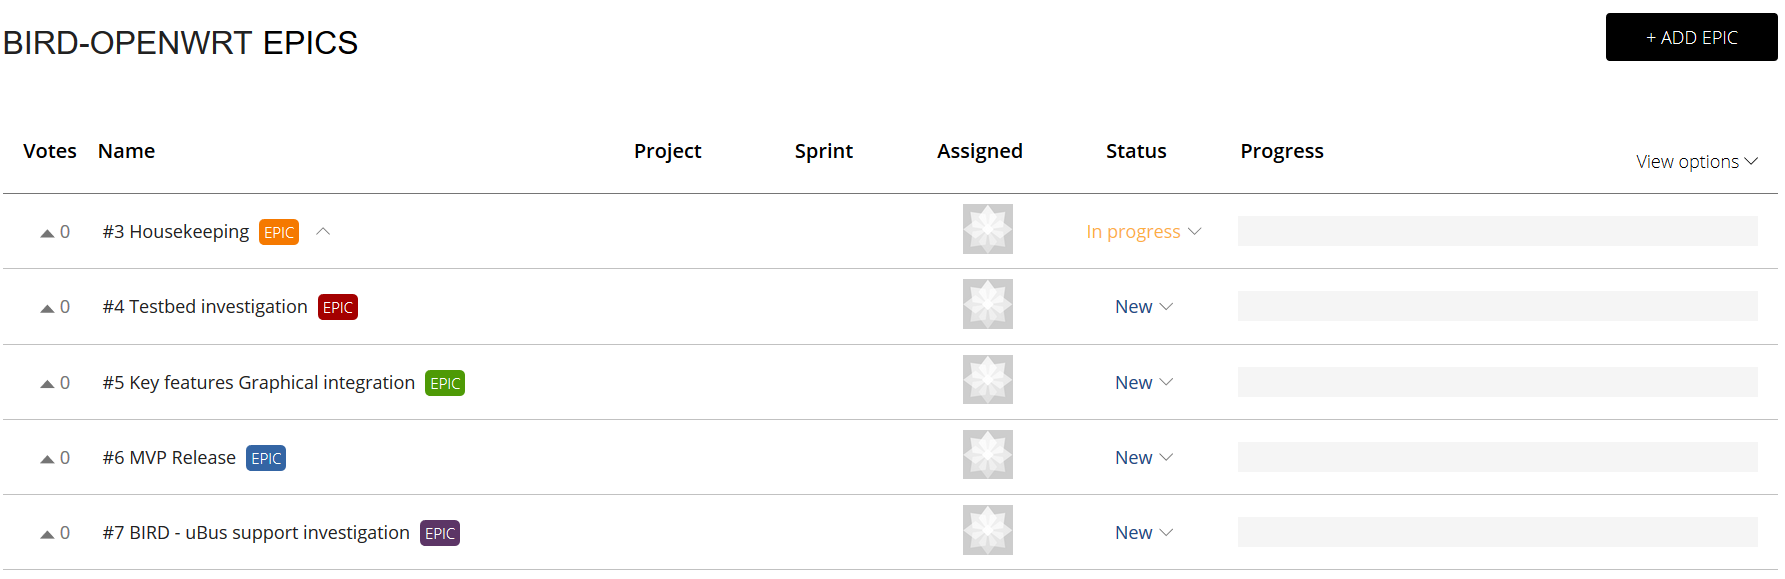
\includegraphics[width=\hsize]{images/kanban/epics}
    \caption{Project EPICs overview}
    \label{fig:kepic}
\end{figure}

This view presents the information about the big tasks represented in project's schedule, who is working on each one, other useful information and how far it is the task of being delivered.
\newpage

\subsection{EPIC Detail View}
\begin{figure}[h!]
\centering
    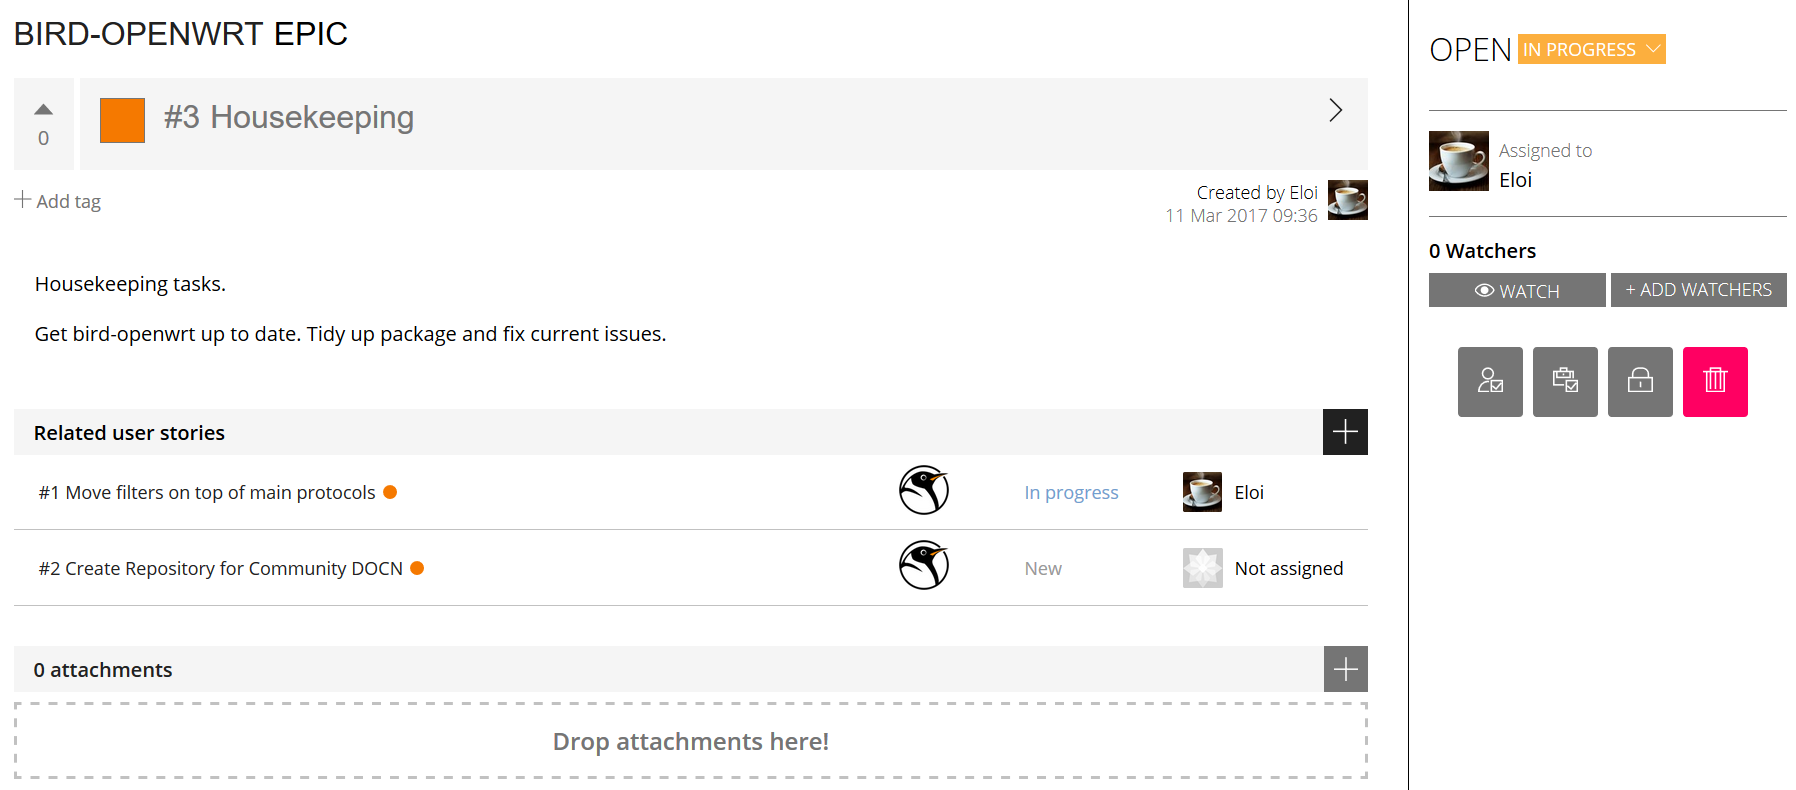
\includegraphics[width=0.85\hsize]{images/kanban/epic-details}
    \caption{Housekeeping EPIC detailed view}
    \label{fig:kepicd}
\end{figure}
This view presents the detailed information of a specific Epic. It presents the first EPIC \textit{Housekeeping} which is In Progress, assigned to \textbf{Eloi} and two tasks, one already in progress and another waiting for resources.
\newpage

\section{Timeline View}
\begin{figure}[h!]
\centering
    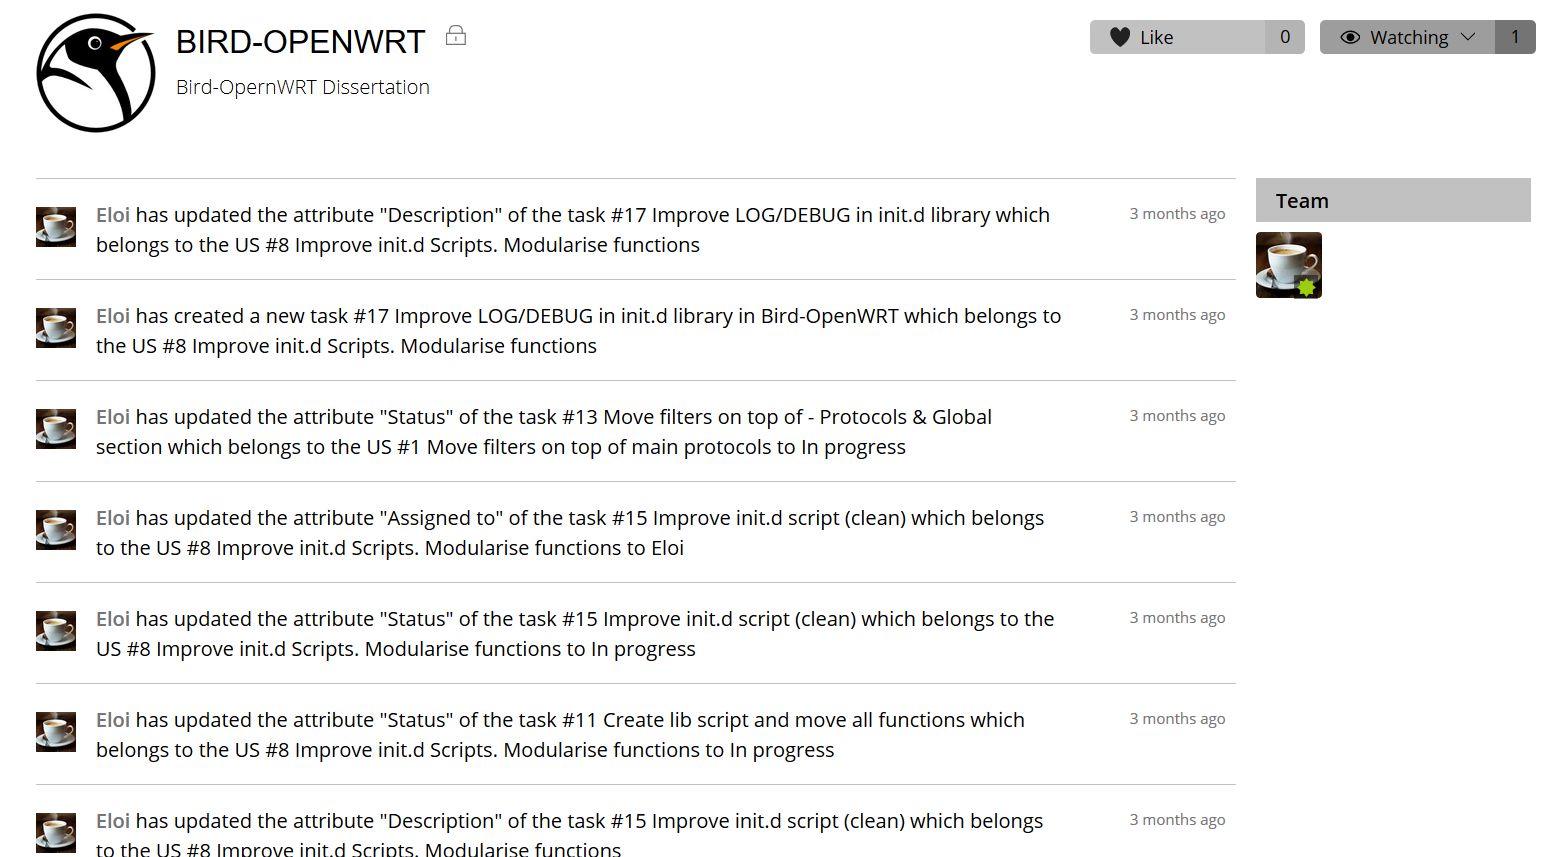
\includegraphics[width=0.7\hsize]{images/kanban/timeline}
    \caption{Project timeline status information}
    \label{fig:ktimeline}
\end{figure}
The Timeline View presents Project's log information. Any action applied to any of the tasks, stories or epics will be logged and shown chronologically in this page.
\newpage

\section{Kanban Board View}
\begin{figure}[ht!]
\centering
    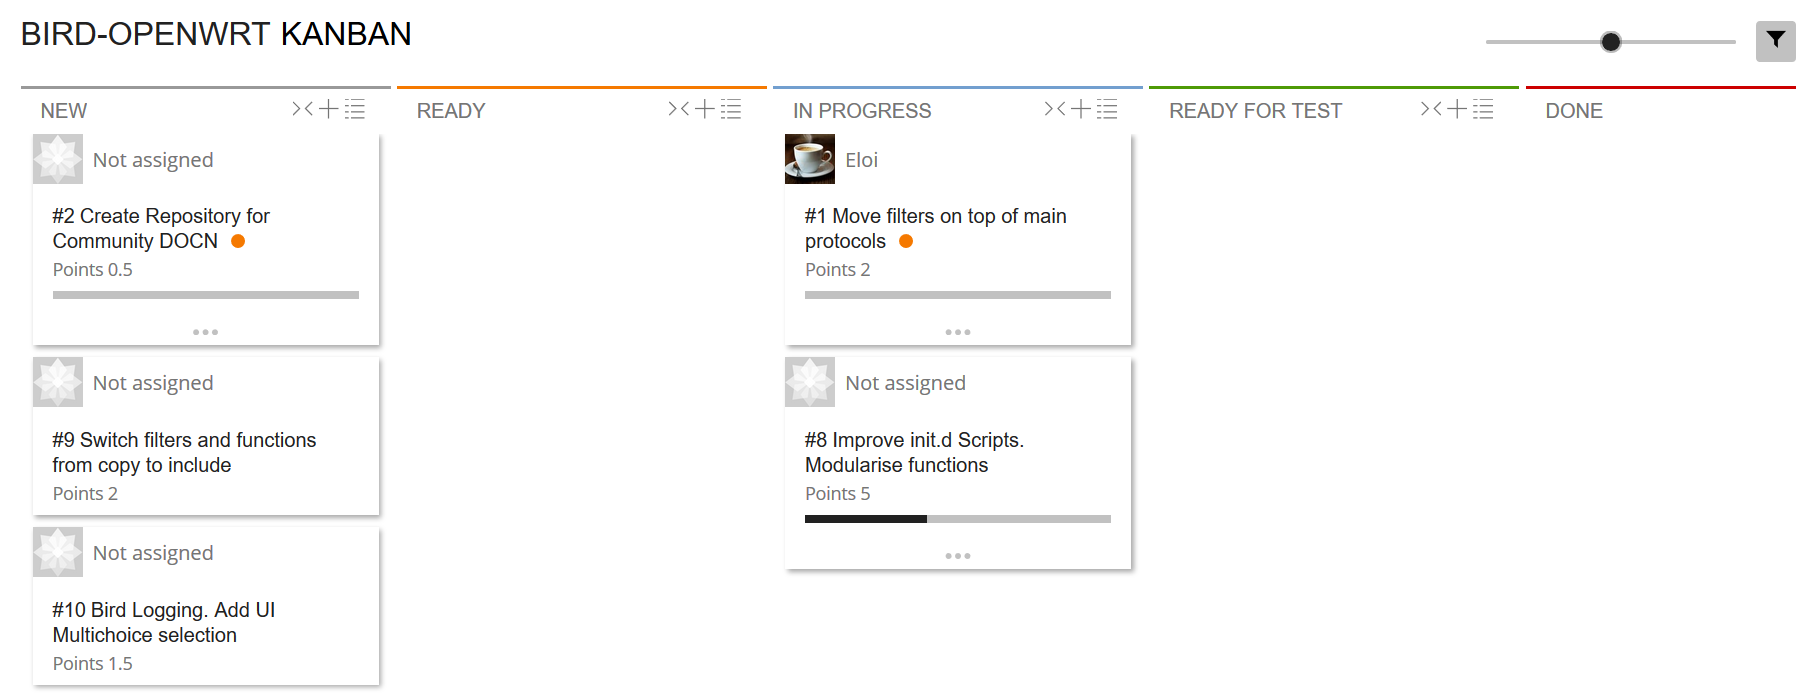
\includegraphics[width=0.85\hsize]{images/kanban/kanban}
    \caption{Kanban User Stories board view}
    \label{fig:kboard}
\end{figure}
The Kanban Board shows the state of the User Stories being addressed, in which state and how far they are from being completed.
\newpage

\subsection{Cycle/Sprint View}
\begin{figure}[ht!]
\centering
    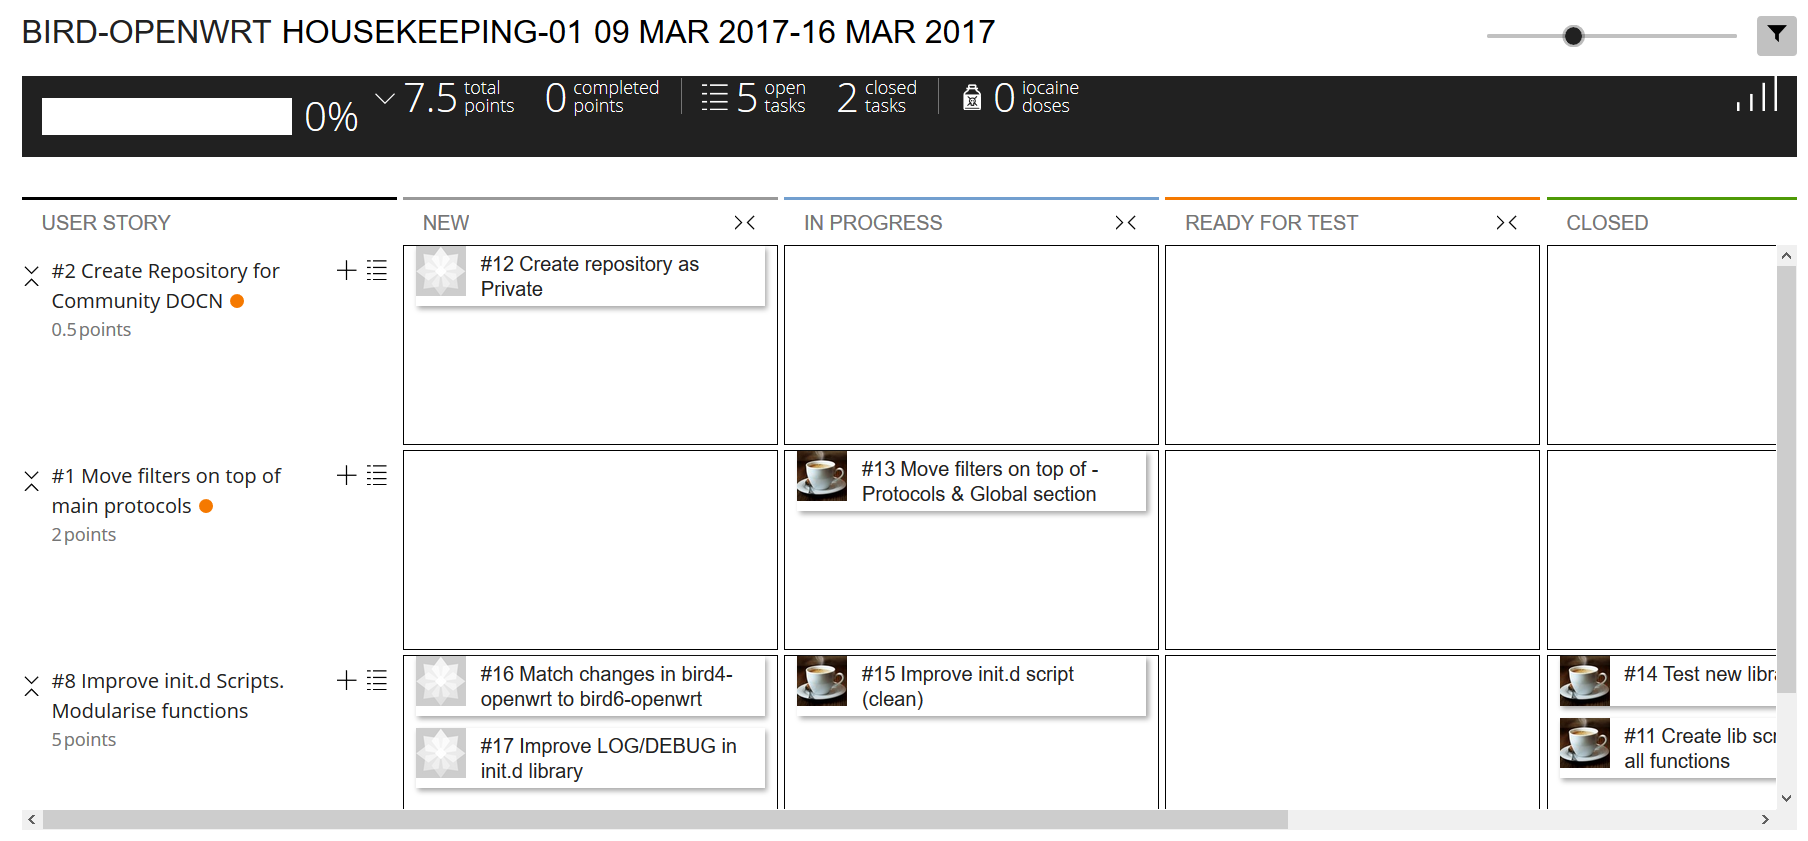
\includegraphics[width=0.85\hsize]{images/kanban/cycle}
    \caption{Kanban current cycle/sprint tasks board view}
    \label{fig:kcycle}
\end{figure}
The Cycle/Sprint View presents the user stories being addressed in priority order (in the left) and all the involved Tasks required to complete each of these user stories, to who are assigned and their state. This is a detailed view of the Kanban Board View.

\end{landscape}

\chapter{Extra LUCI Example Pages}
\label{app:ch:extrap}

\section{Privoxy LUCI2 Status Page}
\begin{figure}[H]
    \centering
    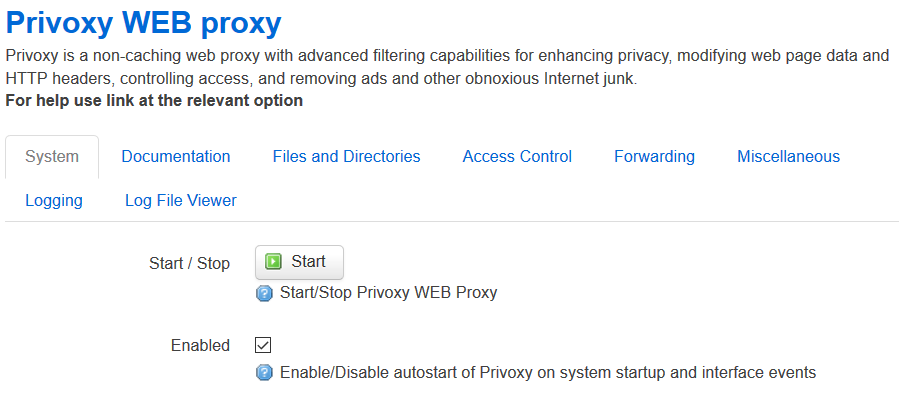
\includegraphics[width=0.95\textwidth]{images/luciextra/disabled}
    \caption{Privoxy \textbf{disabled} service.}
    \label{fig:privdis}
\end{figure}

\begin{figure}[H]
    \centering
    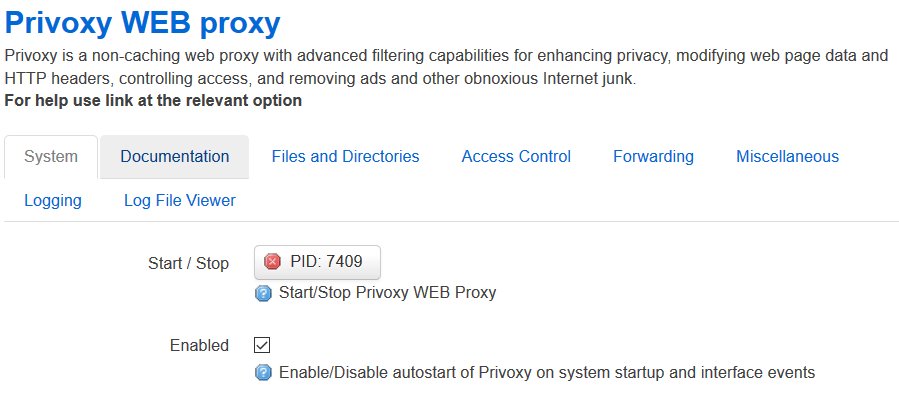
\includegraphics[width=0.95\textwidth]{images/luciextra/enabled}
    \caption{Privoxy \textbf{enabled} service.}
    \label{fig:priven}
\end{figure}
\end{appendices}


\bibliographystyle{ieeetr}
\bibliography{references}
\addcontentsline{toc}{chapter}{{\small Bibliography}}

\end{document}
